\section{Paso 3: Alumno}

  \paragraph{}En última instancia le toca el turno al alumno. Este usuario,
  debe acceder a la aplicación con el nombre de usuario y contraseña con el que
  le fue indicado en el correo electrónico de confirmación de creación de
  usuario, que le fue enviado a su cuenta de correo. La figura
  \ref{capturaPaginaInicial} muestra la página inicial de la aplicación donde se
  debe realizar este acceso.

  \subsection{Respuesta a las preguntas}

  \paragraph{}Para llevar a cabo la realización de la entrevista, el usuario
  alumno debe responder a las preguntas que le fueron propuestas a través de la
  reunión que estableció su asesor. Para ello, debe proceder tal y como se vio
  en el capítulo \ref{responderPreguntas}, \textit{Responder preguntas}. De esta
  forma, el usuario debería ver la captura de pantalla que muestra la figura
  \ref{ejemploRespuestas}.

  \begin{figure}[!ht]
    \begin{center}
      \fbox{
      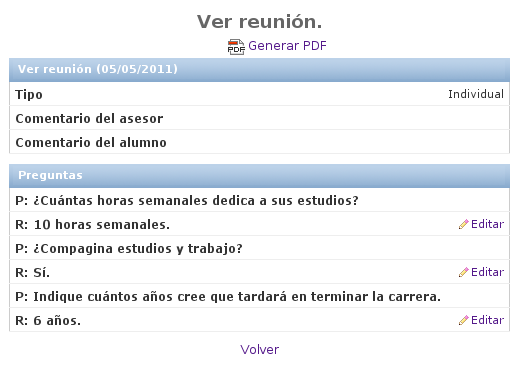
\includegraphics[scale=0.55]{5.Ejemplos_Practicos/5.5.Alumno/ver_respuestas.png}
      }
      \caption{Lista de \textit{Respuestas} de ejemplo.}
      \label{ejemploRespuestas}
    \end{center}
  \end{figure}

  \paragraph{}Una vez respondidas, el usuario \textit{Asesor} podrá ver
  automáticamente las respuestas que le ha dado el alumno al que asesora, con lo
  que podrá tomar decisiones a la hora de realizar la labor de asesoría.